\begin{figure}
\centering

\includegraphics{src/img/laravel-logo-big.png}
\caption{Logo Laravel}
\end{figure}

\#Pourquoi \href{https://laravel.com/}{Laravel} ?

\begin{itemize}
\tightlist
\item
  Framework full stack / glue
\item
  Prise en main rapide
\item
  Bonne documentation, grande \href{http://laravel.io/forum}{communauté}
\item
  Incite au respect des principes
  \href{http://fr.wikipedia.org/wiki/SOLID_(informatique)}{S.O.L.I.D}
\item
  Gratuit et opensource (Licence MIT)
\end{itemize}

\#Historique

\begin{itemize}
\tightlist
\item
  Projet initié en 2011 par \href{http://taylorotwell.com/}{Taylor
  Otwell}
\item
  Basé sur des composants d'autres frameworks
\item
  Mai 2013 : version 4, utilise
  \href{https://getcomposer.org/}{composer}
\item
  Août 2014 : projet PHP le plus
  \href{https://github.com/search?l=PHP\&q=stars\%3A\%3E0\&ref=searchresults\&type=Repositories}{populaire}
  sur github
\item
  \href{http://builtwithlaravel.com/}{Qui} utilise Laravel ?
\item
  version 5.5 sortie en août 2017
\end{itemize}

\#Principales fonctionnalités

\begin{itemize}
\tightlist
\item
  Routes RESTful
\item
  ORM (Eloquent, implémentation du pattern Active Record)
\item
  Migrations
\item
  Moteur de templates (Blade)
\item
  Pagination
\item
  Authentification, sessions
\item
  Mail
\item
  Tests unitaires
\item
  Extensible par \href{http://packalyst.com/}{packages} (bundles) via
  composer
\end{itemize}

\#Le Front Controller

\begin{figure}
\centering
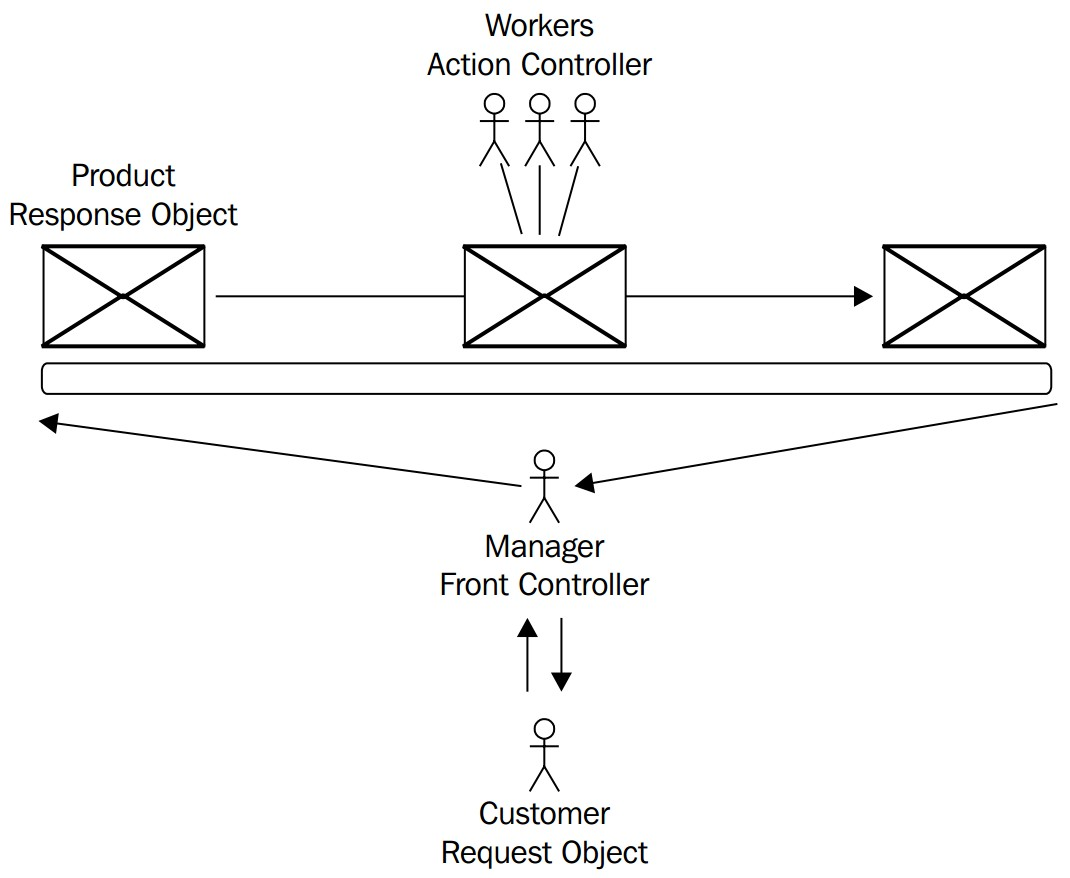
\includegraphics{src/img/front-ctrl.jpg}
\caption{Rôle du front controller}
\end{figure}

\#Architecture

\begin{figure}
\centering
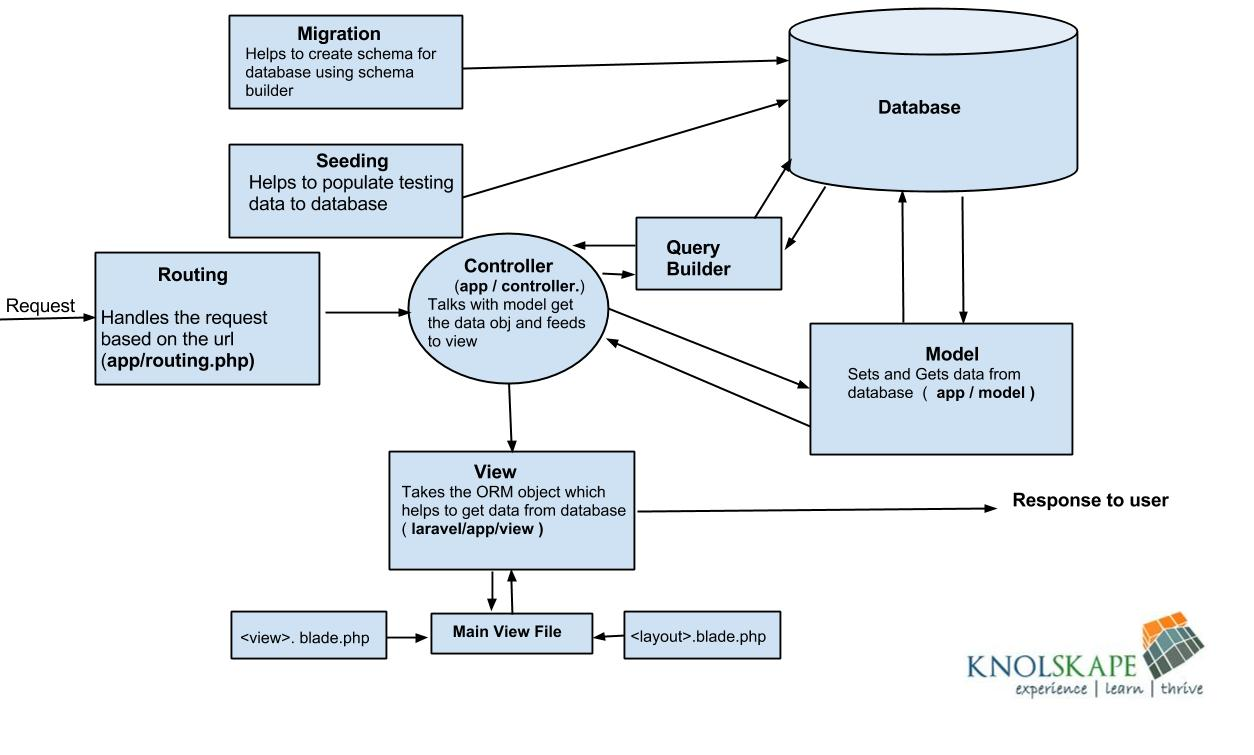
\includegraphics{src/img/laravel-architecture.jpg}
\caption{Architecture de Laravel}
\end{figure}

\#MVC

\begin{itemize}
\tightlist
\item
  Structure d'une appli web =
  \href{https://laravel.com/docs/master/lifecycle}{cycle
  Requête/Reponse}
\item
  Modèle : Eloquent ORM
\item
  Vue : Blade Engine
\item
  Contrôleur : hérite de BaseController
\end{itemize}

\hypertarget{pratique}{%
\section{Pratique}\label{pratique}}

\begin{itemize}
\tightlist
\item
  Conventions de codage : Laravel respecte
  \href{https://laravel.com/docs/5.1/contributions\#coding-style}{PSR-2}

  \begin{itemize}
  \tightlist
  \item
    Vous aussi avec \href{https://styleci.io/}{StyleCI}
  \end{itemize}
\item
  Editeurs et IDE : PhpStorm,
  \href{https://thimble.mozilla.org/fr/}{thimble}, brackets, Sublime
  Text, Atom, \ldots{}
\item
  Tests : unitaires, Jmeter, Selenium, \ldots{}
\item
  Outils : devtools Chrome ou FF, \href{http://emmet.io/}{Emmet}, git
\item
  Doc

  \begin{itemize}
  \tightlist
  \item
    \href{https://laravel.com/docs/master}{Documentation officielle} de
    Laravel
  \item
    \href{http://cheats.jesse-obrien.ca/}{Cheat Sheet}
  \end{itemize}
\item
  Tutoriels

  \begin{itemize}
  \tightlist
  \item
    \href{http://laravel.sillo.org/laravel-5/}{Best Momo},
    \href{https://openclassrooms.com/courses/decouvrez-le-framework-php-laravel-1}{Open
    Classroom},
    \href{https://www.codeschool.com/courses/try-laravel}{CodeSchool}
  \end{itemize}
\end{itemize}

\#Environnement de développement

\begin{itemize}
\tightlist
\item
  Local

  \begin{itemize}
  \tightlist
  \item
    Installation AMP, git + configuration : Long
  \item
    Dépendant du poste de travail
  \item
    Travail offline
  \end{itemize}
\item
  VM (Vagrant - Homestead) ou conteneur

  \begin{itemize}
  \tightlist
  \item
    Mise en route plus rapide : pré-configuré
  \item
    Environnement dédié au dev
  \end{itemize}
\item
  Cloud (cloud9, \ldots{})

  \begin{itemize}
  \tightlist
  \item
    Mise en route plus rapide : pré-configuré
  \item
    Indépendant du poste de travail (navigateur)
  \item
    Outils de synchro disponibles
  \end{itemize}
\end{itemize}

\hypertarget{environnement-de-duxe9veloppement}{%
\section{Environnement de
développement}\label{environnement-de-duxe9veloppement}}

\begin{itemize}
\tightlist
\item
  Cloud:
  \href{https://community.c9.io/t/laravel-5-3-installation-on-cloud9/9038}{Cloud9}
\item
  Local ou VM

  \begin{itemize}
  \tightlist
  \item
    Installer : serveur http, SGBD, git, php7, composer
  \item
    Installer Laravel :
  \end{itemize}
\end{itemize}

\begin{otherlanguage}{english}

\begin{Shaded}
\begin{Highlighting}[]
\VariableTok{$composer} \ExtensionTok{global}\NormalTok{ require }\StringTok{"laravel/installer"}
\end{Highlighting}
\end{Shaded}

\end{otherlanguage}

\hypertarget{duxe9marrer-un-projet}{%
\section{Démarrer un projet}\label{duxe9marrer-un-projet}}

\begin{itemize}
\tightlist
\item
  Créer un nouveau projet
\end{itemize}

\begin{otherlanguage}{english}

\begin{Shaded}
\begin{Highlighting}[]
\NormalTok{$ }\ExtensionTok{composer}\NormalTok{ create-project laravel/laravel raidit}
\CommentTok{# ou si ~/.composer/vendor/bin est dans le PATH :}
\NormalTok{$ }\ExtensionTok{laravel}\NormalTok{ new raidit}
\NormalTok{$ }\BuiltInTok{cd}\NormalTok{ raidit}
\end{Highlighting}
\end{Shaded}

\end{otherlanguage}

\begin{itemize}
\tightlist
\item
  Racine du site dans
  \begin{otherlanguage}{english}\texttt{/public}\end{otherlanguage}
  (lien symbolique ou virtual host)
\end{itemize}

\hypertarget{le-duxe9puxf4t}{%
\section{Le dépôt}\label{le-duxe9puxf4t}}

\begin{itemize}
\tightlist
\item
  Initialiser le dépôt
\end{itemize}

\begin{otherlanguage}{english}

\begin{Shaded}
\begin{Highlighting}[]
\VariableTok{$cd} \ExtensionTok{raidit}
\VariableTok{$git} \ExtensionTok{init}
\VariableTok{$git} \ExtensionTok{add}\NormalTok{ .}
\VariableTok{$git} \ExtensionTok{commit}\NormalTok{ -m }\StringTok{"Install laravel"}
\VariableTok{$git} \ExtensionTok{remote}\NormalTok{ add origin git@github.com:bastian/raidit.git}
\VariableTok{$git} \ExtensionTok{push}\NormalTok{ --set-upstream origin master}
\end{Highlighting}
\end{Shaded}

\end{otherlanguage}

\begin{itemize}
\tightlist
\item
  Penser à ajouter sa clé publique à Github
\end{itemize}

\#\href{https://help.ubuntu.com/lts/serverguide/httpd.html}{Apache}

\begin{itemize}
\tightlist
\item
  Virtual hosts

  \begin{itemize}
  \tightlist
  \item
    \begin{otherlanguage}{english}\texttt{http-vhosts.conf}\end{otherlanguage}
    (activer dans
    \begin{otherlanguage}{english}\texttt{httpd.conf}\end{otherlanguage})
  \item
    Un par site
  \item
    Pointer dans
    \begin{otherlanguage}{english}\texttt{/public}\end{otherlanguage}
  \end{itemize}
\item
  \begin{otherlanguage}{english}\texttt{AllowOverride}\end{otherlanguage}
  : active
  \begin{otherlanguage}{english}\texttt{.htaccess}\end{otherlanguage}
\item
  \begin{otherlanguage}{english}\texttt{.htaccess}\end{otherlanguage} :
  redirection des requêtes
\item
  Alternative : Remplacer le dossier racine http par un lien symbolique
  vers le dossier
  \begin{otherlanguage}{english}\texttt{/public}\end{otherlanguage}
\end{itemize}

\hypertarget{artisan}{%
\section{Artisan}\label{artisan}}

\begin{itemize}
\tightlist
\item
  Laravel's CLI
\item
  Construit avec Symfony Console
\item
  Aide aux tâches courantes, ex:
\end{itemize}

\begin{otherlanguage}{english}

\begin{Shaded}
\begin{Highlighting}[]
\VariableTok{$php} \ExtensionTok{artisan}\NormalTok{ route:list}
\VariableTok{$php} \ExtensionTok{artisan}\NormalTok{ migrate}
\VariableTok{$php} \ExtensionTok{artisan}\NormalTok{ make:controller}

\VariableTok{$php} \ExtensionTok{artisan}\NormalTok{ list}
\end{Highlighting}
\end{Shaded}

\end{otherlanguage}

\begin{itemize}
\tightlist
\item
  \href{https://laravel.com/docs/master/artisan}{Extensible}
\end{itemize}

\hypertarget{premiers-pas}{%
\section{Premiers pas}\label{premiers-pas}}

\begin{itemize}
\tightlist
\item
  \href{https://laravel.com/docs/master/routing}{Routes}

  \begin{itemize}
  \tightlist
  \item
    Ajouter une route
    \begin{otherlanguage}{english}\texttt{/test}\end{otherlanguage}
  \item
    Ajouter un paramètre qui sera affiché :
    \begin{otherlanguage}{english}\texttt{/test/param}\end{otherlanguage}
  \item
    Utiliser une vue pour cette route
  \item
    Lister les routes avec la commande artisan
  \end{itemize}
\end{itemize}

. . .

\begin{itemize}
\tightlist
\item
  \href{https://laravel.com/docs/master/controllers}{Contrôleurs}

  \begin{itemize}
  \tightlist
  \item
    Ajouter un contrôleur :
    \begin{otherlanguage}{english}\texttt{Test}\end{otherlanguage}
  \item
    Lui ajouter une action :
    \begin{otherlanguage}{english}\texttt{index}\end{otherlanguage}
  \item
    Ajouter la route correspondante :
    \begin{otherlanguage}{english}\texttt{/test/index}\end{otherlanguage}
  \end{itemize}
\end{itemize}

. . .

\begin{itemize}
\tightlist
\item
  \href{https://laravel.com/docs/master/views}{Vues}

  \begin{itemize}
  \tightlist
  \item
    Ajouter une vue Blade
    (\begin{otherlanguage}{english}\texttt{.blade.php}\end{otherlanguage})
  \item
    Afficher cette vue dans l'action
    \begin{otherlanguage}{english}\texttt{index}\end{otherlanguage}
  \end{itemize}
\end{itemize}

\hypertarget{ressources}{%
\section{Ressources}\label{ressources}}

\begin{itemize}
\tightlist
\item
  \href{https://laracasts.com/series/laravel-5-fundamentals}{Laracast}
\item
  \href{https://laraveltips.wordpress.com/}{Laravel Tips}
\item
  \href{http://learninglaravel.net/tags/tutorials}{Learning Laravel}
\item
  \href{http://www.tutorials.kode-blog.com/laravel-5-rest-api}{RESTful
  API with Laravel 5}
\item
  \href{https://projets-labinfo.he-arc.ch/projects/webdev/wiki/Ressources_devweb}{Les
  vôtres}
\end{itemize}

\begin{otherlanguage}{english}

\end{otherlanguage}

\hypertarget{sources}{%
\section{Sources}\label{sources}}
